%=========================================================
% Machine Mode MTIME (Memory Mapped)
%=========================================================
\section{Machine Mode MTIME (Memory Mapped)}

Machine Mode MTIME, which is a periodic interrupt timer, is defined as a memory mapped peripheral. The timer counter is 64bit length; its high side is MTIMEH and its lower side is MTIME. The count increment clock source can be selected from the internal system clock or the external clock of the IP. The timer comparator is also 64bit length; its high side is MTIMECMPH and its lower side is MTIMECMP. When the 64bit timer counter matches the timer comparator, an interrupt request is generated. MTIME\_CTRL has the timer enable bit, the clock select bit, the interrupt enable bit and the interrupt status bit. MTIME\_DIV is the pre-scalar configuration of the count clock. MSOFTIRQ can be used to generate IRQ\_SOFT interrupt request.

\begin{table}[H]
    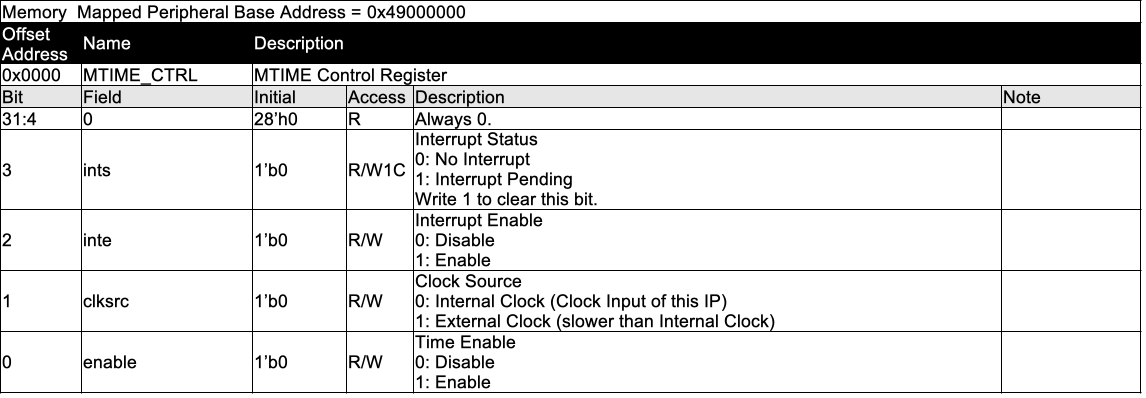
\includegraphics[width=1.00\columnwidth]{./Table/MTIME_CTRL.png}
    \caption{MTIME\_CTRL}
    \label{tb:MTIME_CTRL}
\end{table}

\begin{table}[H]
    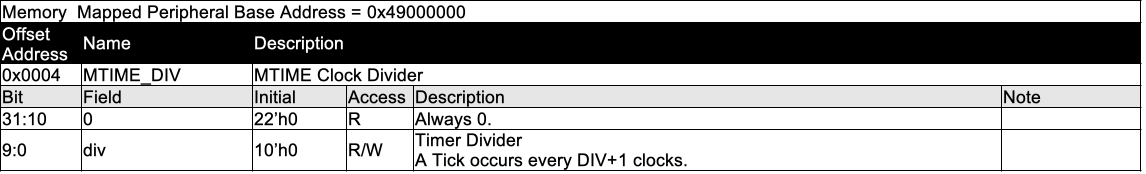
\includegraphics[width=1.00\columnwidth]{./Table/MTIME_DIV.png}
    \caption{MTIME\_DIV}
    \label{tb:MTIME_DIV}
\end{table}

\begin{table}[H]
    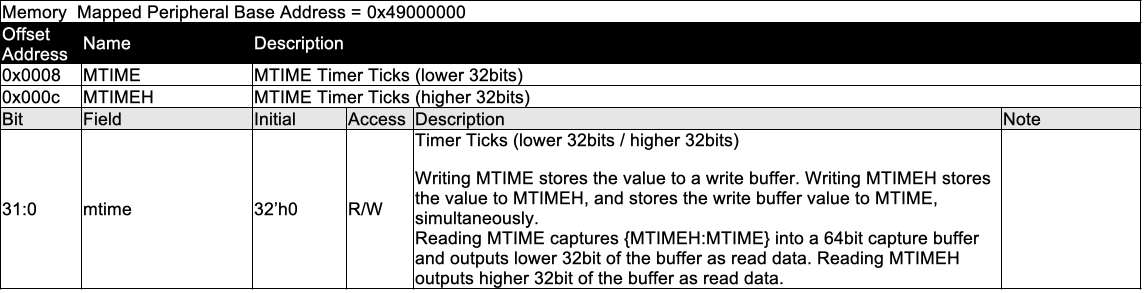
\includegraphics[width=1.00\columnwidth]{./Table/MTIME_TICK.png}
    \caption{MTIME / MTIMEH}
    \label{tb:MTIME_TICK}
\end{table}

\begin{table}[H]
    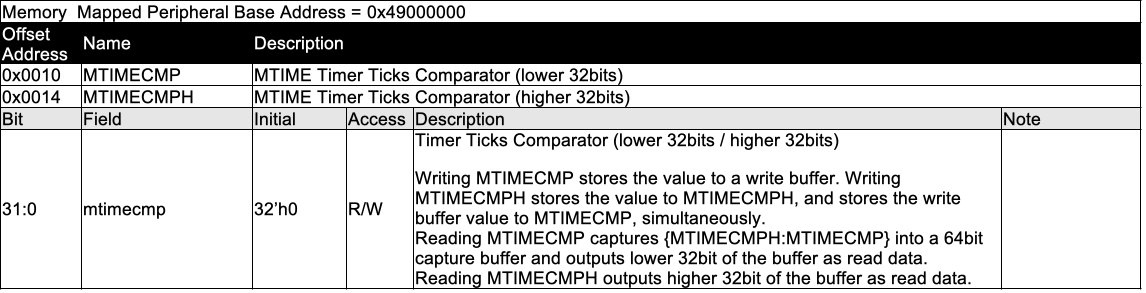
\includegraphics[width=1.00\columnwidth]{./Table/MTIME_CMP.png}
    \caption{MTIMECMP / MTIMECMPH}
    \label{tb:MTIME_CMP}
\end{table}

\begin{table}[H]
    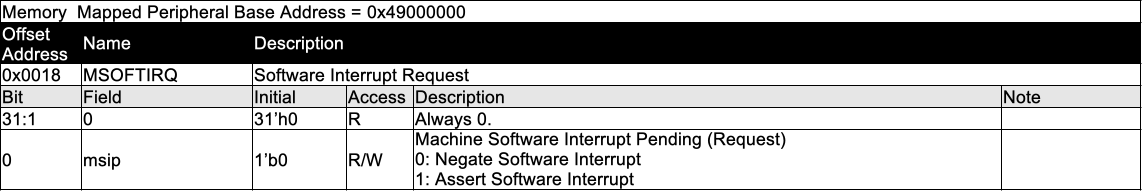
\includegraphics[width=1.00\columnwidth]{./Table/MSOFTIRQ.png}
    \caption{MSOFTIRQ}
    \label{tb:MSOFTIRQ}
\end{table}


